\subsection{Implementando traceroute}

Como dijimos anteriormente, \emph{traceroute} es una herramienta de dignóstico que se utiliza para hacer
un análisis del estado de la conexión entre 2 hosts comunicados a través del protocolo TCP/IP.
Este comando pone especial énfasis en los distintos tramos (determinados por los hops entre routers)
que va debe atravesar el paquete para llegar a destino.
Mediante este tipo de análisis es posible obtener información de gran interés, como por
ejemplo identificar los enlaces con mayor RTT (determinantes en el cálculo del
RTT ''global'', entre el host origen y el destino). De esta manera es posible caracterizar los distintos
enlaces: RTT's altos pueden corresponderse a enlaces submarinos, o de reducida velocidad de transmisión.

La idea básica del algoritmo consiste en enviar paquetes con TTL's incrementales hacia el nodo destino
y obtener información en función de los datagramas ICMP obtenidos, tal como muestra el siguiente
diagrama:

\begin{figure}[!h]
  \begin{center}
      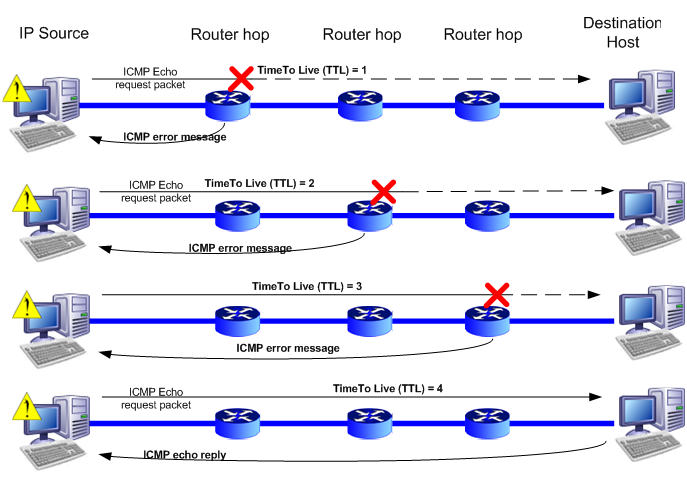
\includegraphics[scale=0.4]{imagenes/traceroute.png}
      \caption{Mecanismo de acción de traceroute}
      \label{fig:contra1}
  \end{center}
\end{figure}

Cada vez que un paquete es forwardeado hacia un router, el valor de su TTL se decrementa en una unidad.
Cuando un routers advierte que el TTL de un paquete ha alcanzado el valor 0, envía un mensaje ICMP hacia
el host fuente del mensaje, de tipo ''time exceeded''. Conociendo la hora exacta de emisión del paquete
original y hora en la cual arriba el mensaje de error es posible determinar el RTT entre el host en el cual se corre el algoritmo
y el router generador del paquete ICMP.
El algoritmo se extiende a cada uno de los nodos intermedios:
En la primera iteración se envía un paquete con valor de TTL 1. Por lo tanto el router a 1 hop de
distancia envía un mensaje de error, y el algoritmo puede calcular el RTT entre el origen y dicho
router.
Generalizando, en la iteración $i$ se envía un paquete con valor de TTL $i$, y utilizando la información
recibida, el algoritmo puede calcular el RTT entre el origen y el router ubicado a $i$ hops.
El algoritmo finaliza o bien cuando se recibe una respuesta afirmativa por parte del destino; o bien
cuando se alcanza el límite de TTL permitido.

\subsubsection{Algunas consideraciones y detalles implementativos}

Para implementar el comando utilizamos la librería \emph{Scapy} de Python.

Traceroute por default envía una secuencia de paquetes UDP hacia el nodo destino. Paquetes del estilo
TCP SYN también pueden ser usados. En nuestra implementación la alternativa utilizada son los paquetes
ICMP de tipo ''echo request'' . Los mensajes recibidos serán por lo tanto del tipo ''time exceeded''
para los nodos intermedios y ''echo reply'' cuando el paquete llega a destino.

La función debe recibir como argumentos el valor de TTL inicial con el que envía el primer paquete
y el máximo de saltos permitidos hasta alcanzar el destino. En nuestro caso utilizamos los valores
por defecto: 1 y 30 respectivamente.

Otro de los parámetros que debe especificarse es el número de reintentos que debe realizarse por cada
valor de TTL. ICMP, al igual que IP, es una capa ''sin garantías'' en el envío de mensajes. Los routers
hacen el ''mejor esfuerzo'' para lograr el envío de los paquetes, pero no hay garantías de que los mismos
alcancen el destino.
Teniendo esto en cuenta, es posible que los mensajes ICMP enviados por los routers no lleguen al emisor.
En dicho caso, es deseable que se realice más de un intento para un determinado valor de TTL.
Usualmente la mayoría de las implmentaciones utilizan 2 o 3 como valor. En nuestro caso decidimos
realizar 10 intentos por cada TTL. Este valor nos protege contra otro aspecto sensible del algoritmo,
descripto a continuación.

Un paquete no llega al mismo destino atravesando siempre las mismas rutas. Los nodos intermedios pueden
caerse o levantarse. Determinados enlaces pueden congestionarse o liberarse en distintos momentos.
Supongamos que el algoritmo envía hacia el destino un paquete con TTL 10. ¿Qué garantías tenemos de que,
en caso de ser necesario un segundo intento porque no ha llegado ningún mensaje de error, el router
alcanzado luego del décimo hop sea el mismo? Ninguna. En otras palabras, dependiendo la ruta que siga
el datagrama, el router alcanzado luego del décimo hop será uno u otro.
Para tener cierto control respecto a esta situación, por cada valor de TTL se envían 10 paquetes y
se guardan todas las direcciones de IP que han respondido los mensajes de error.
Luego, el algoritmo selecciona aquella dirección que ha respondido más veces.

Finalmente, el valor de RTT entre el host que corre el \emph{traceroute} y el router a $i$ hops de
distancia es calculado como el promedio de los valores obtenidos por cada intento.

\subsection{Zscore}

Más especificamente, \textcolor{red}{estimamos un RTT promedio} para cada salto que se da en
la ruta que nos comunica con cada host, y \textcolor{red}{normalizamos este valor para
conseguir un ZRTT} para cada salto que nos de suficiente informaci\'on como para
\textcolor{red}{analizar el trasfondo del tr\'afico en la red}.

